\documentclass[twocolumn]{aastex631}


\shorttitle{LSST Pipelines Software}
\shortauthors{LSST Data Management Pipeline Developers}

\begin{document}

\title{The LSST Pipelines Software}

\AuthorCallLimit=999
\input{authors}

\begin{abstract}

The Vera C.\ Rubin Observatory will produce the Legacy Survey of Space and Time (LSST) and produce 11 data releases over the ten-year survey.
The LSST Science Pipelines Software will be used to create these data releases and to perform the nightly alert.
This paper provides an overview of the LSST Science Pipelines Software and describes the components and how they are combined to form pipelines.

\end{abstract}


\keywords{%
    Astrophysics - Instrumentation and Methods for Astrophysics
    ---
    methods: data analysis
    ---
    methods: miscellaneous
}

\section{Introduction}

The Large Synoptic Survey Telescope \citep[LSST;][]{2008arXiv0805.2366I} is an 8.4\,m telescope being built on Cerro Pachon in Chile.
The Data Management System \citep[DMS;][]{2015arXiv151207914J} is designed to handle the flow of data from the telescope, approaching 20\,TB per night, in order to issue alerts and to prepare annual data releases.
A central component of the DMS is the LSST Science Pipelines software that provides the algorithms and frameworks required to process the data and generate the coadds, difference images, and catalogs to the user community for scientific analysis.

The LSST Science Pipelines software consists of the building blocks required to construct high performance pipelines to process the data from LSST.
It has been under development since at least 2004 \citep{2004AAS...20510811A} and has evolved significantly over the years as the project transitioned from prototyping \citep{2010SPIE.7740E..15A} and entered into formal construction \citep{2018SPIE10707-10J}.
The software is designed to be usable by other optical telescopes and this has been demonstrated with Hyper Suprime Cam \citep{2018PASJ...70S...5B}.

In this paper we provide an overview of the components of the software system.
This includes a description of the support libraries and data access abstraction, along with the algorithmic components and the pipeline task system.
We do not include validation of the individual algorithms.
The other components of the LSST DMS, such as the workflow system, the Qserv database \citep{Wang:2011:QDS:2063348.2063364} and the LSST Science Platform \citep{LSE-319}, are described elsewhere.

\section{Fundamentals}
\label{sec:support}

The LSST Science Pipelines software is written in Python with C++ used for high-performance algorithms and for core classes that are usable in both languages.
We use Python 3 \citep[having ported from python 2,][currently with a minimum version of Python 3.12]{2020ASPC..522..541J}, and the C++ layer can use C++17 features with pybind11 being used to provide the interface from Python to C++.
Additionally, the C++ layer uses \texttt{ndarray} to allow seamless passing of C++ arrays to and from Python \texttt{numpy} arrays.
This compatibility with \texttt{numpy} is important in that it makes LSST data structures available to standard Python libraries such as Scipy and Astropy \citep{2016SPIE.9913E..0GJ,2018AJ....156..123A}.

Although all the software uses the \texttt{lsst} namespace, the code base is split into individual Python products in the LSST GitHub organization\footnote{\url{https://github.com/lsst}} that can be installed independently and which declare their own dependencies.
These dependencies are managed using the ``Extended Unix Product System'' \citep[EUPS;][]{EUPS,2018SPIE10707E..09J} where
most of the products are built using the SCons system \citep{2005Scons1377085} with LSST-specific extensions provided in the \texttt{sconsUtils} package enforcing standard build rules and creating the necessary Python package metadata files.

For logging we always use standard Python logging with an additional \texttt{VERBOSE} log level between \texttt{INFO} and \texttt{DEBUG} to provide additional non-debugging detail that can be enabled during batch processing.
This verbose logging is used for periodic logging where long-lived analysis tasks are required to issue a log message every 10 minutes to indicate to the batch system that they are still alive and actively performing work.
For logging from C++ we use Log4CXX wrapped in the \texttt{lsst.log} package to make it look more like standard Python logging, whilst also supporting deferred string formatting such that log messages are only formed if the log message level is sufficient for the message to be logged.
These C++ log messages are forwarded to Python rather than being issued from an independent logging stream.
Finally, we also provide some LSST-specific exceptions that can be thrown from C++ code and caught in Python.

As of April 2025, the Science Pipelines software is approximately 700,000 lines of Python and 225,000 lines of C++.
The number of lines in the pipelines code as a function of time is given in Fig.~\ref{fig:pipe-loc}.

\begin{figure}
\plotone{fig-pipe-loc}
\caption{The number of lines of code comprising the LSST Science Pipelines software as a function of year.
Line counts include comments but not blank lines. Python interfaces are implemented using \texttt{pybind11} and that is counted as C++ code. For the purposes of this count Science pipelines software is defined as the \texttt{lsst\_distrib} metapackage and does not include code from third party packages.}
\label{fig:pipe-loc}
\end{figure}

\subsection{Python environment}

An important aspect of running a large data processing campaign is to ensure that the software environment is well defined.
We define a base python environment using conda-forge via a meta package named \texttt{rubin-env}\footnote{\url{https://github.com/conda-forge/rubinenv-feedstock}}.
This specifies all the software needed to build and run the science pipelines software.
A Docker container is built for each software release and the fully-specified versions of all software are recorded to ensure repeatability.

\subsection{Unit Testing and Code Coverage}

Unit testing and code coverage are critical components of code quality \citep{2018SPIE10707E..09J}.
Every package comes with unit tests written using the standard \texttt{unittest} module.
We run the tests using \texttt{pytest} \citep{pytest} and this comes with many advantages in that all the tests run in the same process and requiring global parameters to be well understood, tests can be run in parallel in multiple processes, plugins can be enabled to extend testing and record test coverage, and a test report can be created giving details of run times and test failures.
Coding standards compliance with PEP\,8 \citep{pep8} is enforced using GitHub Actions, the \texttt{ruff} package, and \texttt{pre-commit} checks.
A Jenkins system provides the team with continuous integration facilities that includes running longer tests with pre-cursor datasets.

\section{Data Access Abstraction}
\label{sec:data-access}

\subsection{Butler}

Early in the development of the LSST Science Pipelines software it was decided that the algorithmic code should be written without knowing where files came from, what format they were written in, where the outputs are going to be written or how they are going to be stored.
All that the algorithmic code needs to know is the relevant data model and the Python type.
To meet these requirements we developed a library called the Data Butler \citep[see e.g.,][]{2022SPIE12189E..11J,2023arXiv230303313L}.

The Butler internally is implemented as a registry, a database keeping track of datasets, and a datastore, a storage system that can map a Butler dataset to a specific collection of bytes.
A datastore is usuall a file store (including POSIX file system, S3 object stores, or WebDAV) but could also be implemented as a NoSQL database or a metrics database such as Sasquatch \citep{SQR-068}.

\begin{deluxetable}{ll}

%% Keep a portrait orientation

%% Over-ride the default font size
%% Use Default (12pt)

%% Use \tablewidth{?pt} to over-ride the default table width.
%% If you are unhappy with the default look at the end of the
%% *.log file to see what the default was set at before adjusting
%% this value.

%% This is the title of the table.
\tablecaption{Common dimensions present in the default dimension universe.\label{tab:dims}}

%% This command over-rides LaTeX's natural table count
%% and replaces it with this number.  LaTeX will increment
%% all other tables after this table based on this number
%% \tablenum{1}

%% The \tablehead gives provides the column headers.  It
%% is currently set up so that the column labels are on the
%% top line and the units surrounded by ()s are in the
%% bottom line.  You may add more header information by writing
%% another line between these lines. For each column that requries
%% extra information be sure to include a \colhead{text} command
%% and remember to end any extra lines with \\ and include the
%% correct number of &s.
\tablehead{\colhead{Name} & \colhead{Description} \\
\colhead{} & \colhead{} }

%% All data must appear between the \startdata and \enddata commands
\startdata
\texttt{instrument} &  Instrument.  \\
\texttt{band} & Waveband of interest.  \\
\texttt{physical\_filter} &  Filter used for the exposure. \\
\texttt{day\_obs} & The observing day. \\
\texttt{group} &  Group identifier. \\
\texttt{exposure} & Individual exposure. \\
\texttt{visit} &  Collection of 1 or 2 exposures. \\
\texttt{tract} &  Tesselation of the sky. \\
\texttt{patch} &  Patch within a tract.\\
\enddata

%% Include any \tablenotetext{key}{text}, \tablerefs{ref list},
%% or \tablecomments{text} between the \enddata and
%% \end{deluxetable} commands

\end{deluxetable}

A core concept of the Butler is that every dataset must be given what we call a ``data coordinate.''
The data coordinate locates the dataset in the dimensional space where dimensions are defined in terms that scientists understand.
Some commonly used dimensions are listed in Table~\ref{tab:dims}.
Each dataset is uniquely located by specifying its dataset type, its run collection, and its coordinates, with Butler refusing to accept another dataset that matches all three of those values.
The dataset type defines the relevant dimensions and the associated Python storage class.
The run collection can be thought of as a folder but does not have to be a folder within datastore.

As a concrete example, the file from one detector of an LSSTCam observation taken sometime in 2025 could have a data coordinate of \texttt{instrument="LSSTCam", detector=42, exposure=2025080300100} and be associated with a \texttt{raw} dataset type.
The \texttt{exposure} record itself implies other information such as the physical filter and the time of observation.
A deep coadd on a patch of sky would not have \texttt{exposure} dimensions at all and would instead be something like \texttt{instrument="LSSTCam", tract=105, patch=2, skymap="something"}, which would tell you exactly where it is located in the sky since you can calculate it from the tract and patch and skymap.

\subsection{Instrument Abstractions: Obs Packages}
\label{sec:obs_packages}

The Butler and pipeline construction code know nothing about the specifics of a particular instrument.
In the default dimension universe there is an \texttt{instrument} dimension that includes a field containing the full name of a Python \texttt{Instrument} class.
This class, which uses a standard interface, is used by the system to isolate the instrument-specific from the pipeline-generic.
Some of the responsibilities are:

\begin{itemize}
\item Register instrument-specific dimensions such as \texttt{detector}, \texttt{physical\_filter} and the default \texttt{visit\_system}.
\item Define the default \texttt{raw} dataset type and the associated dimensions.
\item Provide configuration defaults for pipeline task code that is processing data from this instrument.
\item Provide a ``formatter'' class that knows how to read raw data.
\item Define the default curated calibrations known to this instrument.
\end{itemize}

By convention we define the instrument class and associated configuration in \texttt{obs} packages.
As an extension to the base definition of an ``instrument``, the LSST Science Pipelines define a modified \texttt{Instrument} class that includes focal plane distortions using the \texttt{afw} package (see \S\ref{sec:afw}).
There are currently project-supported \texttt{obs} packages for:

\begin{itemize}
\item LSSTCam \citep{2024SPIE13096E..1SR,2024SPIE13096E..1OL, 2024SPIE13103E..0WU,2010SPIE.7735E..0JK}, LATISS \citep{2020SPIE11452E..0UI}, and associated Rubin Observatory test stands and simulators.
\item Hyper-SuprimeCam \citep{2018PASJ...70S...1M}.
\item The Dark Energy Camera \citep{2015AJ....150..150F,2008SPIE.7014E..0ED}.
\item CFHT's MegaPrime \citep{2003SPIE.4841...72B}.
\end{itemize}

Additionally, teams outside the project have developed \texttt{obs} packages to support Subaru's Prime Focus Spectrograph \citep{2020SPIE11447E..7VW}, VISTA's VIRCAM \citep{2015A&A...575A..25S},
the Wide Field Survey Telescope \citep[WFST;][]{2025arXiv250115018C}, and the Gravitational-wave Optical Transient Observer \citep[GOTO;][]{2021PASA...38....4M}.

\subsection{Metadata Translation}

Every instrument uses different metadata standards but the Butler data model and pipelines require some form of standardization to determine values such as the coordinates of an observation, the observation type, or the time of observation.
To perform that standard extraction of metadata each supported instrument must provide a metadata translator class using the \texttt{astro\_metadata\_translator} infrastructure.\footnote{\url{https://astro-metadata-translator.lsst.io}}
The translator classes can understand evolving data models and allow the standardized metadata to be extracted for the lifetime of an instrument even if headers changed.
Furthermore, in addition to providing standardized metadata the package can also provide programmatic or per-exposure corrections to data headers prior to calculating the translated metadata.
This allows files that were written with incorrect headers to be recovered.

\subsection{Application Framework}
\label{sec:afw}
\texttt{afw} -- this is called the ``Application Framework'' in \citet{2010SPIE.7740E..15A}\footnote{This document can be downloaded from \url{https://ls.st/Document-9349}}

\begin{itemize}
\item Image/MaskedImage/Exposure
\item Table and Catalogs.
\item Detection
\item Math
\item Camera geometry
\item FITS I/O
\item WCS: AST library \citep{2016A&C....15...33B} backs the world coordinate system handling.
\end{itemize}

\section{Instrument Signature Removal}
\label{sec:isr}

\subsection{Amplifier Offset Correction}
\label{sec:isr:ampoffset}
The amplifier offset correction (commonly referred to as amp-offset correction, or pattern continuity correction) runs as part of the instrument signature removal (ISR) process.
This correction is designed to address systematic discontinuities in background sky levels across amplifier boundaries.
We believe that these discontinuities arise from electronic biases between adjacent amplifiers, persisting even after application of dark and flat corrections.

Drawing on the \texttt{PANSTARRS}' Pattern Continuity algorithm \citep{2020ApJS..251....4W}, our method aims to eliminate these offsets, thereby preventing problems such as background over-/under-subtraction at amplifier boundaries caused by discontinuities across the detector.

The amp-offset algorithm initially computes a robust flux difference measure between two narrow strips along each amplifier-amplifier interface.
Regions containing detected sources, or pixel data which have been masked for other reasons, are not considered.
These amp-interface differences are stored in an amp-offset matrix; diagonal entries represent the number of neighboring amplifiers, and off-diagonal entries encode information about the associations between amplifiers.
A complementary interface matrix encodes directional information for these associations.
Using this information, a least-squares minimization is performed to determine the optimal pedestal value to be added or subtracted to each amp which would reduce the amp-offset between that amplifier and all of its neighboring amplifiers.
This method is generalized to support 2D amplifier geometries within a detector, as with LSSTCam, incorporating length-based weighting into the matrices to account for amplifiers that are not square.
\section{Measurement System}

Measurement plugin system.

\texttt{meas\_base} and \texttt{meas\_algorithms}


\subsection{meas\_deblender}
\subsection{meas\_extensions\_convolved}
\subsection{meas\_extensions\_gaap}
\subsection{meas\_extensions\_photometryKron}
\subsection{meas\_extensions\_piff}
\subsection{meas\_extensions\_psfex}
\subsection{meas\_extensions\_scarlet}
\subsection{meas\_extensions\_shapeHSM}
\subsection{meas\_extensions\_simpleShape}
\subsection{meas\_extensions\_trailedSources}
\subsection{meas\_modelfit}
\subsection{meas\_transiNet}

\section{Difference Imaging}
\label{sec:diffim}

Difference imaging is implemented in \texttt{ip\_diffim}, and is divided into three steps.
First, a base template image is constructed with \texttt{getTemplate} by warping previously-generated coadded images to the WCS and bounding box of the science image.
Then the warped template is subtracted from the science image using one of several available algorithms in \texttt{subtractImages}, which produces a temporary difference image.
Finally, peaks are detected on the difference image and DiaSources are measured in \texttt{detectAndMeasure}.
The final difference image with updated mask planes is written along with the DiaSource catalog.

\subsection{subtractImages}

The primary implementation of image subtraction used by \texttt{subtractImages} is based on \cite{1998ApJ...503..325A}, and uses spatially-varying Gaussian basis functions for the fit.
The PSF-matching kernel can be constructed for either the science or the template image, and the resulting difference image is decorrelated \citet{DMTN-021}.
Optionally, the science image can be preconvolved with its own PSF before PSF-matching, producing a Score image analogous to \citet{2016ApJ...830...27Z}.

\subsection{detectAndMeasure}

Positive and negative peaks are detected by thresholding the Score image if it is available.
Otherwise, the difference image is smoothed with a Gaussian of the same width as the PSF of the science image, and thresholds are taken on the smoothed image.
Contiguous pixels around each peak that are statistically brighter than the background are grouped into source footprints, and any overlapping footprints are merged.
Footprints that contain both a positive and a negative peak are fit as dipoles.
The dipole fit simultaneously solves for the negative and positive lobe centroids and fluxes using non-linear least squares minimization.
DiaSources that are not classified as dipoles instead fall back on an SDSS-style centroid \citep{2003AJ....125.1559P}.
Finally, all configured measurement plugins are run, including HSM shape measurements \citep{2003MNRAS.343..459H,2005MNRAS.361.1287M} and trailed source measurements.

\section{Astrometric and Photometric Calibration}
\label{sec:jointcal}

\subsection{Astrometric Calibration}

\texttt{meas\_astrom}
\texttt{gbdes} \citep{2022ascl.soft10011B,2017PASP..129g4503B}

Jointcal no longer discussed.

\subsection{Photometric Calibration}

\subsection{fgcmcal}

FGCM \citep{2018AJ....155...41B}

\section{Pipelines}
\label{sec:pipe}

\subsection{Pipeline Support}

The \texttt{Task} Python class provides a standard interface for how to execute an algorithm.
The \texttt{PipelineTask} variant provides stronger guarantees on configuration and provides a means by which the pipeline execution framework can determine how to link a task into a pipeline and how to determine what type of data should be read from a Butler and what should be written out to a Butler.

Describe \texttt{pex\_config} because it's not described anywhere.

Pipeline in YAML.

Show plot of a simple pipeline visualization.

Graph building.

Show plot of a graph where a pipeline now includes specific datasets as inputs.

Describe that provenance is stored in the output files and in the graph itself.

Execution system and how BPS provides the interface between a quantum graph and a workflow system.


\subsection{Task library}

\subsubsection{\texttt{pipe\_tasks}}

\subsubsection{\texttt{drp\_tasks}}


\subsection{Pipeline Collections}

\subsection{Calibration pipelines}
\label{sec:calib_pipe}

The high-level pipelines to build calibration products (\texttt{cp}) for the LSST cameras are defined in \texttt{cp\_pipe}.
They set ISR (see \secref{sec:isr}) configuration parameters needed for each calibration product, by enabling all the sequential steps of the ISR task up to the step before the correction being generated.
In some cases, configurations also specify whether to combine exposures (for bias or dark exposures for instance) and to bin exposures to support diagnostic displays.

Once calibration products are produced, they are ``verified'' (see \citet{DMTN-222} for more details) using \texttt{cp\_verify} pipelines by checking they pass metrics defined in \citet{DMTN-101}.
In this case, verify configuration parameters enable all corrections in the ISR task up to and including the application of the correction being verified. As a result, the calibration products can then be certified to be available in the Butler and used to ISR an exposure.

\subsubsection{\texttt{drp\_pipe}}

\subsection{\texttt{ap\_pipe}}

The \texttt{ap\_pipe} package defines the pipeline(s) to be used for real-time Alert Production processing \citep{DMTN-219}.
These pipelines include instrument signature removal (\S\ref{sec:isr}), calibration (\S\ref{}), measurement plugins (\S\ref{sec:meas}), image differencing (\S\ref{sec:dia}), source association (\S\ref{sec:association}), and alert generation (\S\ref{sec:alerts}).
Some of these tasks are shared with the pipelines in \texttt{drp\_pipe}, but configured to prioritize speed over strict quality; for example, they use a minimal set of measurement plugins.

\texttt{ap\_pipe} currently has pipeline variants for LSSTCam, LSSTComCam, LATISS, the Rubin Observatory simulators, Hyper-SuprimeCam, and the Dark Energy Camera.
Because these variants serve as testbeds for AP-specific algorithms and configuration settings, they are, as much as possible, the ``same'' pipeline, differing almost entirely in loading instrument defaults from \texttt{obs} packages (\S\ref{sec:obs_packages}).
The only other customization is an extra task for handling DECam's inter-chip crosstalk, which does not have an equivalent for Rubin instruments.


\section{Catalog Schemas}
\label{sec:schemas}

Must transform pipeline products from the internal data model to the public data model defined in \citet{LSE-163}.

\texttt{sdm\_schemas}
\texttt{felis}

\subsection{Display Abstractions}
\label{sec:display}

The \texttt{afw.display} subpackage defines a simple image display abstraction layer that be used to show our image objects via multiple applications and libraries.
This includes programmatic control of stretch levels and colors, WCS mapping, semi-transparent bitmask overlays, and simple geometric region support.

There are currently implementations for matplotlib \citep{2007CSE.....9...90H}, Firefly \citep{2020ASPC..527..243R}, SAOImage DS9 \citep{2003ASPC..295..489J}, and Ginga \citep[][via Astrowidgets]{2013ASPC..475..319J}.
While most of these tools have considerable functionality beyond what our abstraction layer provides, the ability to interact easily with them in a consistent, programmatic way in many different contexts (e.g., DS9 on personal machines, matplotlib and Ginga in Jupyter notebooks, and Firefly in the Rubin Science Platform) is invaluable, and usually the minimal \texttt{afw.display} interface provides all we need.

\section{Data Analysis}
\label{sec:analysis}

\texttt{analysis\_tools}

The analysis_tools package provides a framework to allow reproducible, automatic creation of plots and metrics through a set of configurable, reusable tools that can be used in pipeline execution and interactive analysis.
The package allows metrics and plots to be consistently created at various points in the pipeline and ensures that the metrics dispatched to the monitoring dashboard (better word?) are generated in sync with the archived plots.
The package was designed to handle the large data volumes and memory requirements that the survey will generate to ensure that the initial QA products required are rapidly made and readily available for fast action on any emergent data quality issues.
The individual tools run in the pipelines to calculate the metrics can then be reused in an interactive environment, such as a script or notebook, allowing further investigation into arising issues to reproduce exactly what was originally run.

\texttt{verify}

\texttt{faro} --- \textbf{do not document this as we are no longer using it for primary metrics calculation}.

\subsection{Validating the Science Pipelines}
\label{sec:validation}

We use small, of order of a few gigabyte, datasets that can be processed as part of continuous integration.
These take of order an hour to process.
There are regular re-processings of standard datasets that can take a few days to process.
For formal data releases there are additional metrics calculated and a test report is issued, such as the one made available with release 28.0 \citep{DMTR-451}.

TODO: Mention CI packages like ci\_imsim and ci\_hsc here, as referenced from schemas section.

\subsection{Source Injection}
\label{sec:source_injection}

The \texttt{source\_injection} package contains tools designed to assist in the injection of synthetic sources into scientific imaging.
Source injection is a powerful tool for testing the algorithmic performance of the LSST Science Pipelines, generating measurements on synthetic sources where the truth is known and facilitating subsequent quality assurance checks.
Synthetic source generation and injection capability is provided by the \textsc{GalSim} software package \citep{2015A&C....10..121R}.
An example showcasing the injection of a series of synthetic Sérsic sources into an HSC i-band image is shown in Figure \ref{fig:source_injection_example}.

\begin{figure}
    \centering
    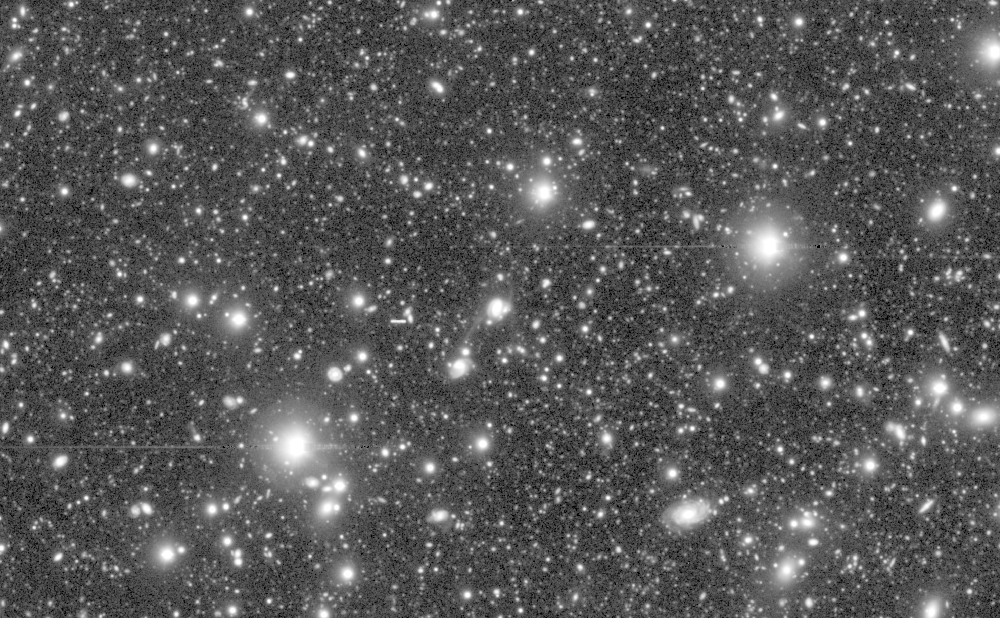
\includegraphics[width=\linewidth]{figures/analysis/source_injection/t9813p42i_zoom_sersic_pre_injection}
    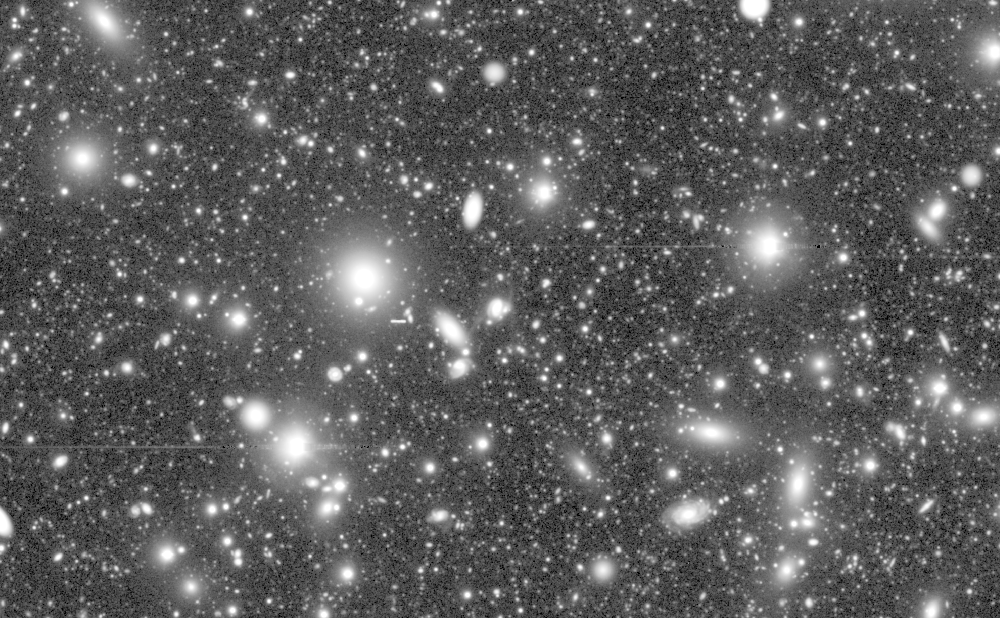
\includegraphics[width=\linewidth]{figures/analysis/source_injection/t9813p42i_zoom_sersic_post_injection}
    \caption{
        An HSC i-band cutout from tract 9813, patch 42, showing before (top) and after (bottom) the injection of a series of synthetic Sérsic sources.
        Images are ~100 arcseconds on the short axis, log scaled across the central 99.5\% flux range, and smoothed with a Gaussian kernel of FWHM 3 pixels.
    }
    \label{fig:source_injection_example}
\end{figure}

Synthetic sources can be injected into any imaging data product output by the LSST Science Pipelines, including visit-level exposure-type or visit-type datasets (i.e., datasets with the dimension \texttt{exposure} or \texttt{visit}), or into a coadd-level coadded dataset.
These injection tasks are defined in \texttt{ExposureInjectTask}, \texttt{VisitInjectTask} and \texttt{CoaddInjectTask}, respectively.
Each task operates similarly: read in an injection catalog containing the parameters of the sources to be injected, generate sources using \textsc{GalSim}, and inject them into the input image.
An additonal mask plane (\texttt{INJECTED} by default) is appended to the image mask to identify pixels which have been touched by injected sources.
Optional modifications to the noise profiles of injected sources and the variance plane of the image can also be performed.

With \textsc{GalSim} we have the capacity to generate synthetic sources of varying profile types, including Gaussian, exponential and Sérsic profiles \citep{1963BAAA....6...41S, 1968adga.book.....S}, each convolved with the local PSF.
We also have the option to inject scaled versions of the PSF model itself in order to simulate stars.
If preferred, a pre-generated FITS image of a source can be injected instead of a model generated by \textsc{GalSim}, allowing for the injection of complex sources or postage stamp cutouts of real data.

Alongside the primary injection tasks, a suite of helper tools are also provided to optionally assist in the generation of synthetic source catalogs and injection pipelines.
Fully qualified source injection pipeline definition YAML files are normally constructed using an existing pipeline as a baseline reference.
A user specifies which dataset type they would like to inject synthetic sources into, and the \texttt{source\_injection} package generates a new pipeline definition YAML file that includes the correctly configured source injection task.
By default, all tasks in the pipeline downstream of the point at which source injection occurs are modified such that their connection names are prefixed with \texttt{injected\_}.
This ensures that an injected dataset is not confused with the original dataset when stored together in a common collection.

Once source injection has completed, the source injection task will output two dataset types: an injected image, and an associated injected catalog.
The injected image is a copy of the original image with the injected sources added.
The injected catalog is a catalog of the injected sources, with the same schema as the original catalog and additional columns describing per-source source injection success outcomes.


\section{Conclusions}


\begin{acknowledgments}
This material is based upon work supported in part by the National Science Foundation through Cooperative Agreement AST-1258333 and Cooperative Support Agreement AST-1202910 managed by the Association of Universities for Research in Astronomy (AURA), and the Department of Energy under Contract No. DE-AC02-76SF00515 with the SLAC National Accelerator Laboratory managed by Stanford University.
Additional Rubin Observatory funding comes from private donations, grants to universities, and in-kind support from LSSTC Institutional Members.
\end{acknowledgments}

\facility{Rubin}
\software{%
ndarray\footnote{\url{https://github.com/ndarray/ndarray}},
astropy \citep{2022ApJ...935..167A},
pytest \citep{pytest},
matplotlib \citep{2007CSE.....9...90H},
galsim \citep{2015A&C....10..121R},
numpy \citep{Harris2020},
}

\bibliography{local,lsst,lsst-dm,refs_ads,refs,books}

\end{document}
